
\documentclass[a4paper,lithuanian]{article}

\usepackage[utf8]{inputenc}
\usepackage[L7x]{fontenc}
\usepackage[lithuanian]{babel}
\usepackage{graphicx}
\graphicspath { {./} }

\title{MU5 Kompiuterio techninis aprašymas}

\author{
  Adam Jasinski\\
  VU MIF, Bioinformatika, II kursas
}

\begin{document}

\maketitle

\newpage

\section{Įvadas}

MU5 yra penkta kompiuterio sistema suprojektuota ir pastatyta Mančesterio Universitete nuo 1946 metų. Praeiti Mančesterio universiteto darbai, ypač \\Manchester Mark 1 ir Atlas turėjo didelę reikšmę industrijoje ir moksle. Praeitos mašinos buvo sukurtos Elektrinės inžinerijos skyriaus nariais ir bendradarbiavimo tarp universiteto ir vietinės industrijos, ypač Ferranti Ltd.. 1964 metais, buvo suformuota atskira informatikos katedra, kurios tikslu buvo reikšminga mokslinės veiklos plėtra, pradedant pirmųjų metų informatikos absolventais, 1968 metais. Tuo metu, universitetas naudojo anksčiau minėtą Atlas kaip skaičiavimų vykdymo sistemą, ir iš patirties buvo nuspręsta, kad aparatūros ir programinės įrangos mokslinė veikla negali būti efektyviai atliekama naudojant viso universiteto naudojamą skaičiavimų vykdymo sistemą. To rezultatu buvo reikmė nepriklausomai įrangai mokslinės veiklos vykdymui, bet labiau noras tęsti pažangių sistemų sistemų projektavimą ir statymą ir novatoriškos idėjos, kurios vėliau galėtų būti išnaudojamas kompiuterių industrijos.\newline

1968 sausį, po kelių metų diskusijų, MU5 projektui buvo suteikta £630.446 mokslinė stipendija, kurios pakako tik mažai versijai (architektūriniu mastu) potencialiai didelės sistemos. Fiziškai, MU5 buvo didelė mašina, ką galite pamatyti 1 pav.\newline



\begin{figure}[h]
	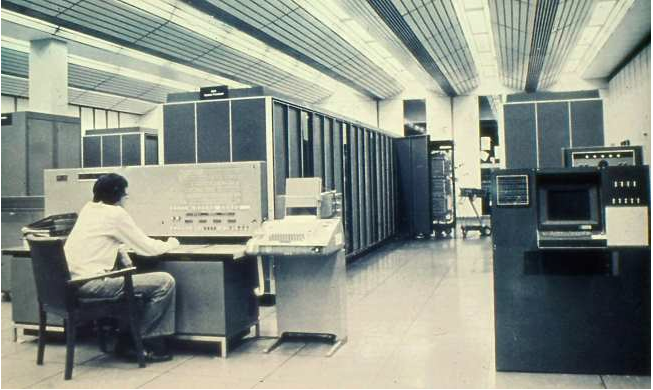
\includegraphics[scale=0.4]{mu5-room}
	\centering
	\caption{MU5 kambarys, su jo operatoriumi prie konsolės}
	\label{}
\end{figure}

MU5 paleidimo darbai prasidėjo 1971 vasarą, o pilnai veikti pradėjo 1974 vidury, kai atsirado galimybė leisti Algol ir Fortran programas. Praeiti Mančesterio Universiteto kūriniai turėjo tiesioginį komercinį atitikmenį, kai MU5 tokio neturėjo, bet turėjo didelę įtaką ICL 2900 serijos kompiuterių architektūrai, kurioje tvarkos kodas, adresavimo struktūra ir operandų formos skiriasi tik smulkmenomis nuo MU5. \newline

Pilnai veikiantis MU5 kompiuteris teikė skaičiavimų vykdymo paslaugą iki 25 aktyvių vartotojų vienu metu, iki kol nebuvo išrinktas 1982 metais.




\section{Rezultatai ir aptarimas}

Pagrindiniai rezultatai. Nuoroda į pav.~\ref{amin}.



Tekstas... Nuoroda į \ref{tab} lentelę ir į \ref{another-tab} lentelę.

\begin{table}[ht]
  \caption{Lentelės pavyzdys}
  \label{tab}
  \begin{tabular}{|l|l|l|l|}
    \hline
    Stulpelio antraštė & Stulpelis II & Stulpelis III & Stulpelis IV \\
    \hline
    Duomenys & duomenys & duomenys...  & ir t.t... \\
    \hline
  \end{tabular}
\end{table}

\begin{table}[ht]
  \caption{Kita lentelė}
  \label{another-tab}
  \begin{tabular}{|l|l|l|l|}
    \hline
    Stulpelio antraštė & Stulpelis II & Stulpelis III & Stulpelis IV \\
    \hline
    Duomenys & duomenys & duomenys...  & ir t.t... \\
    \hline
  \end{tabular}
\end{table}

%% \bibliographystyle{plain}
%% \bibliography{citations}

\end{document}
